\documentclass{revtex4-2}
\usepackage[english]{babel}
\usepackage{graphicx} % Required for inserting images
\usepackage{amsmath}
\usepackage{amsthm}
\usepackage{amssymb}
\usepackage{braket}
\usepackage{tikz}
\usepackage[compat=0.6]{yquant}
\usepackage{nicematrix}
\usepackage{algorithm}
\usepackage{algpseudocode}

\usetikzlibrary{fit,quotes}
\usetikzlibrary{trees}

\pgfdeclareshape{yquant-multictrlshape}{
   \inheritsavedanchors[from=yquant-circle]%
   \foreach \anc in {center, north, north east, east, south east, south, south west, west, north west} {%
      \inheritanchor[from=yquant-circle]{\anc}%
   }%
   \inheritanchorborder[from=yquant-circle]%
   \backgroundpath{%
      \pgfpathmoveto{\pgfqpoint{-0.707107\dimexpr\xradius\relax}{-0.707107\dimexpr\yradius\relax}}%
      \pgfpathlineto{\pgfqpoint{0.707107\dimexpr\xradius\relax}{0.707107\dimexpr\yradius\relax}}%
      \pgfpathellipse{\pgfpointorigin}%
                     {\pgfqpoint{\xradius}{0pt}}%
                     {\pgfqpoint{0pt}{\yradius}}%
   }%
   \inheritclippath[from=yquant-circle]%
}


\pgfdeclareshape{yquant-varmultictrlshape}{
   \inheritsavedanchors[from=yquant-circle]%
   \foreach \anc in {center, north, north east, east, south east, south, south west, west, north west} {%
      \inheritanchor[from=yquant-circle]{\anc}%
   }%
   \inheritanchorborder[from=yquant-circle]%
   \backgroundpath{%
      \pgfpathmoveto{\pgfqpoint{-0.707107\dimexpr\xradius\relax}{-0.707107\dimexpr\yradius\relax}}%
      \pgfpathlineto{\pgfqpoint{0.707107\dimexpr\xradius\relax}{0.707107\dimexpr\yradius\relax}}%
      \pgfpathellipse{\pgfpointorigin}%
                     {\pgfqpoint{\xradius}{0pt}}%
                     {\pgfqpoint{0pt}{\yradius}}%
   }%
   \behindbackgroundpath{%
      \begin{pgfscope}
         % Shift to the center and move up by 1.2 times the yradius
         \pgftransformshift{\pgfqpoint{0pt}{\dimexpr-1\yradius\relax}}
         % Scale the tilde
         \pgftext[center,base]{\scalebox{1.4}{$\tilde{}$}}
      \end{pgfscope}
   }%
   \inheritclippath[from=yquant-circle]%
}


\yquantset{multictrl/.style={every negative control/.style={draw, /yquant/default fill,shape=yquant-multictrlshape,radius=1.05mm}}}

\yquantset{multictrlpos/.style={every positive control/.style={draw, /yquant/default fill,shape=yquant-multictrlshape,radius=1.05mm}}}

\yquantset{varmultictrl/.style={/yquant/every control/.style={shape=yquant-varmultictrlshape,radius=1.05mm}}}

\yquantset{plusctrl/.style={/yquant/every control/.style={/yquant/operators/every not}, every positive control/.style={}}}



\begin{document}

One of the principle challenges in quantum computing is the data loading problem as efficient quantum algorithms can become bottlenecked by the cost of preparing their input states. For example, given a state of interest $\sum_{x=0}^{2^n-1} c_x \ket{x}$ we may try to naively prepare it through $2^n$ rotation gates, and hence any algorithm that runs faster than $2^n$ becomes a subdominant cost. However, if there is some underlying structure to the state we wish to encode we can make use of compression techniques to load the state more efficiently. For example, the uniform superposition state $\ket{+}^{\otimes n}$ can be prepared with just $n$ Hadamard gates (an exponential speed up on naive state preparation).

Piecewise polynomial approximations are one of many classical compression techniques used for storing time series data. In this work we utilise these approximations to efficiently load the amplitudes of quantum states. Previous work \cite{mcardleQuantumStatePreparation2022, gonzalez-condeEfficientAmplitudeEncoding2023} demonstrated how QSVT can be used to load states whose amplitudes are given by functions that can be closely approximated by a global polynomial. We extend this by inventing techniques to apply separate polynomials to different segments of amplitudes.

An important limitation of our approach is that the pieces we split our domain into must correspond to ignoring bits of $x$. This means that all the pieces must be $2^l$ in size and must start with a value divisible by $2^l$ for some integer $l$. In this work we let $l_{x}$ specify the value of $l$ for the piece that $x$ lies in, $m_{x}$ specify the index of the piece that $x$ lies in.

In order to carry out this piecewise QSVT it is necessary to find a diagonal block encoding $U$ with $x$-th entry given by $\frac{x \mod 2^{l_x}}{2^{l_x}}$. The following circuit efficiently performs such a block encoding upon two entangled registers $\ket{x}\ket{l_x}$.
\begin{equation}
\begin{tikzpicture}
\begin{yquant}

% qubit {parity bit} hb;
qubit {flag} flag1;
qubit {flags} flags;
qubit {$\ket{x}$} block;
qubit {$\ket{l_x}$} l;
qubit {control} flag2;

["north:$N$" {font=\protect\footnotesize, inner sep=0pt}]
slash block;

["north:$L_{max}$" {font=\protect\footnotesize, inner sep=0pt}]
slash flags;

["north:$l_{max}$" {font=\protect\footnotesize, inner sep=0pt}]
slash l;

[multictrl]
box {$U_{l_x}$} ( flag1, flags, block)|  flag2 ~ l;

text {$=$} (-);

["north:$N$" {font=\protect\footnotesize, inner sep=0pt}]
slash block;

["north:$L_{max}$" {font=\protect\footnotesize, inner sep=0pt}]
slash flags;

["north:$l_{max}$" {font=\protect\footnotesize, inner sep=0pt}]
slash l;

x flag1;
h flag1;

h flags;


align -;
text {$\ket{-}$} flag1;
text {$\ket{k}$} flags;
text {$\ket{x}$} block;
% text {$\ket{+}$} hb;

[multictrl]
box {high bit\\ add} (block, flags, flag1) |  flag2 ~ l;

% z hb;



text {$\ket{k }$} flags;
text {$\ket{x }$} block;
text {$\frac{(-1)^a}{\sqrt{2}}\ket{a \oplus (k_l+x_l\ge 2^{l_x}) }$} flag1;

h flag1;
x flag1;

% cnot flag1 | hb;
% h hb;
h flags;
\end{yquant}
\end{tikzpicture}
\end{equation}
This high bit add computes the carry bit from adding the first $l$ bits of $x$ ($x_l = x \mod 2^{l}$) and $k$ ($k_l = k \mod 2^{l}$) where the value of $l$ comes from the control register. 

Proof that this is a block encoding of the desired matrix:
% \begin{equation}(\bra{0}\otimes\bra{0}\otimes\bra{x}\otimes\bra{l_x}) U (\ket{0}\otimes\ket{0}\otimes\ket{x}\otimes\ket{l_x}) =  \frac{1}{L_{max}}\sum_{k=0}^{L_{max}-1} \delta((k_{l_x}+x_{l_x})\ge 2^{l_x}) = \frac{1}{2^{l_x}}\sum_{k=0}^{2^{l_x}-1} \delta((k+x_{l_x})\ge 2^{l_x}) = \sum_{k=2^{l_x}-x_{l_x}}^{2^{l_x}-1} \frac{1}{2^{l_x}} = \frac{x_{l_x}}{2^{l_x}}
% \end{equation}
\begin{align}(\bra{0}\otimes\bra{0}\otimes\bra{x}\otimes\bra{l_x}) U (\ket{0}\otimes\ket{0}\otimes\ket{x}\otimes\ket{l_x}) &=  \frac{1}{2L_{max}}\sum_{a=0}^1\sum_{k=0}^{L_{max}-1} (-1)^a (-1)^{a \oplus ((k_{l_x}+x_{l_x})\ge 2^{l_x}))}\\
&= \frac{1}{L_{max}}\sum_{k=0}^{L_{max}-1}  (-1)^{(k_{l_x}+x_{l_x})\ge 2^{l_x})}\\
&= \frac{1}{2^{l_x}}\sum_{k=0}^{2^{l_x}-1} (-1)^{(k+x_{l_x})\ge 2^{l_x})} \\
&= \sum_{k=0}^{2^{l_x}-x_{l_x}} \frac{1}{2^{l_x}}-\sum_{k=2^{l_x}-x_{l_x}}^{2^{l_x}-1} \frac{1}{2^{l_x}} = \frac{2^{l_x}-2x_{l_x}}{2^{l_x}}\\
&= 1 - 2\frac{x \mod 2^{l_x}}{2^{l_x}}
\end{align}

This high bit add can be performed using unary iteration \cite{babbushEncodingElectronicSpectra2018} and a quantum adder \cite{gidneyHalvingCostQuantum2018}. The following circuit illustrates this procedure for when $l_{max} = 3$:
\begin{equation*}
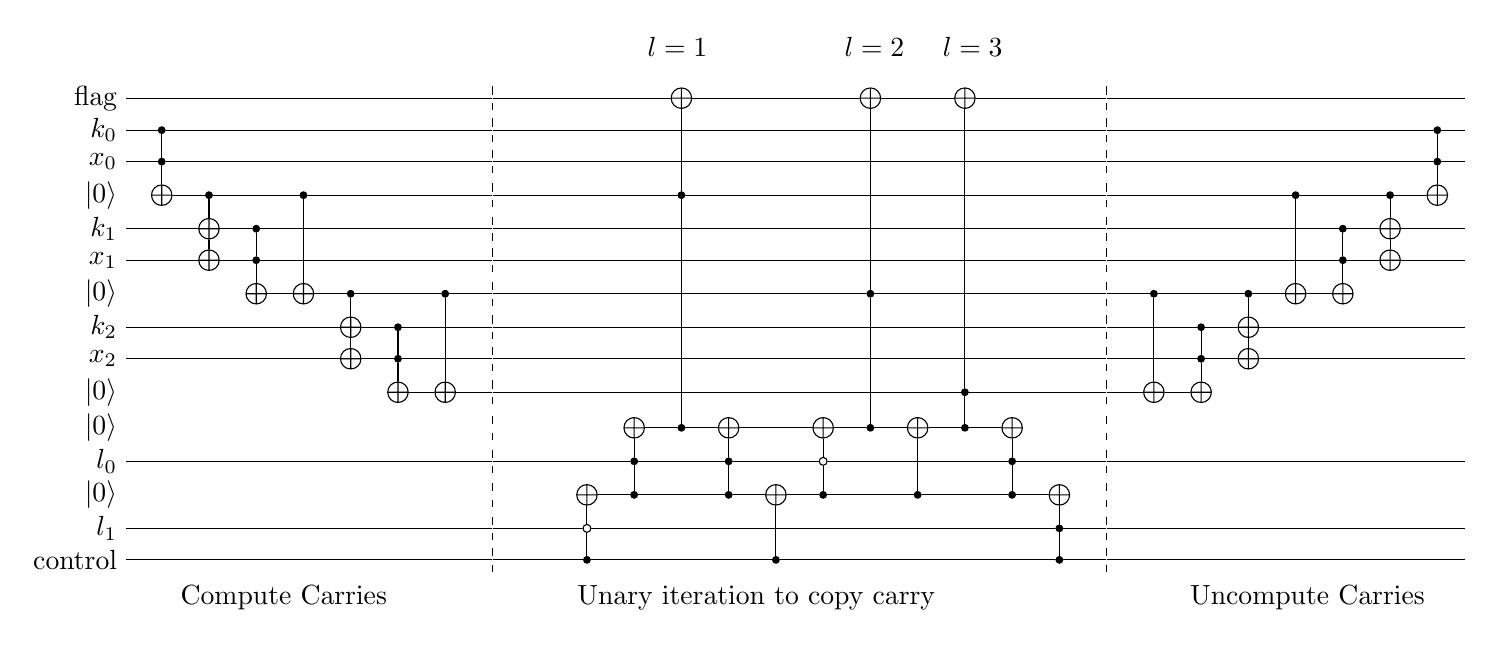
\begin{tikzpicture}
\begin{yquant}

qubit {flag} f;






qubit {$k_{0}$} k0;
qubit {$x_{0}$} x0;
qubit {$\ket{0}$} c0;
discard c0;
hspace {-0.5cm} -;

qubit {$k_{1}$} k1;
qubit {$x_{1}$} x1;
qubit {$\ket{0}$} c1;
discard c1;


qubit {$k_{2}$} k2;
qubit {$x_{2}$} x2;
qubit {$\ket{0}$} c2;
discard c2;

qubit {$\ket{0}$} anc1;
discard anc1;
qubit {$l_{0}$} l1;
qubit {$\ket{0}$} anc0;
discard anc0;
qubit {$l_{1}$} l0;



qubit {control} flag;

setstyle {|-, shorten <= 0.5cm} c0;
init {} c0;
cnot c0 | x0, k0;


cnot x1, k1 | c0;

setstyle {|-, shorten <= 1.3cm} c1;
init {} c1;

cnot c1 | k1, x1;
cnot c1 | c0;

cnot x2, k2 | c1;
setstyle {|-, shorten <= 3cm} c2;
init {} c2;

cnot c2 | k2, x2;
cnot c2 | c1;


barrier l0, l1, flag, anc0, anc1, x0, k0, x1, k1, x2, k2, c0, c1, c2, f;

setstyle {|-, shorten <= 0.5cm} anc0;
init {} anc0;
cnot anc0 | flag ~l0 ;

setstyle {|-, shorten <= 1.1cm} anc1;
init {} anc1;
cnot anc1 | anc0 ,l1 ;

cnot f | c0, anc1;

cnot anc1 | anc0, l1;
cnot anc0 | flag;
cnot anc1 |  anc0 ~ l1;
cnot f | c1, anc1;
cnot anc1 | anc0;
cnot f | c2, anc1;

cnot anc1 | anc0 , l1;
discard anc1;
cnot anc0 | flag, l0;
discard anc0;
barrier l0, l1, flag, anc0, anc1, x0, k0, x1, k1, x2, k2, c0, c1, c2, f;
cnot c2 | c1;
cnot c2 |  k2, x2;
discard c2;
cnot x2, k2 | c1;


cnot c1 | c0;
cnot c1 | k1, x1;
discard c1;
cnot x1, k1 | c0;

cnot c0 |  x0, k0;
discard c0;

\end{yquant}
\node at (2,-6.5) {Compute Carries};
\node at (8,-6.5) {Unary iteration to copy carry};
\node at (15,-6.5) {Uncompute Carries};
\node at (7,0.5) {$l=1$};
\node at (9.5,0.5) {$l=2$};
\node at (10.75,0.5) {$l=3$};
\end{tikzpicture}
\end{equation*}
The unary iteration \cite{babbushEncodingElectronicSpectra2018} controls a copy from the carry bits into the flag register, so the correct carry bit is copied down depending on the input $l$. The calculation of each carry bit is performed via a slightly modified version of the adder circuit described in \cite{gidneyHalvingCostQuantum2018}. We have removed the final addition layer and made the uncompute symmetrical to the compute for clarity.


The addition and the unary iteration each cost $l_{max}$ compute/uncompute Toffoli pairs, whilst the copy operations cost $l_{max}$ Toffolis.  Therefore, the total cost for a $l_{max}$-high bit adder is $15l_{max}$ T-gates.

Now we have block encoding $U$ of piecewise monotonic sequences we can apply piecewise QSVT to this block encoding to produce a piecewise polynomial transformation of our block encoding $U$. This is illustrated by the following circuit (shown for $4$ iterations = $2d$) which applies a different polynomial to each segment of diagonal block encoding
\begin{equation}
\begin{tikzpicture}
\begin{yquant}
qubit {flag} flag1;
qubit {flags} flags;
qubit {$x$} n;
qubit {anc0} l;



slash flags;

["north:$N$" {font=\protect\footnotesize, inner sep=0pt}]
slash n;

["north:$l_{max}$" {font=\protect\footnotesize, inner sep=0pt}]
slash l;
h flag1;

[varmultictrl]
box {load $l_x$} l ~ n;


[varmultictrl]
box {$R_z(\phi_{0,m_{x}})$} flag1 ~ n;

cnot flags ~ flag1;
[multictrlpos]
box {$U_{l_x}$} (flags, n)  | l ~ flag1;


[varmultictrl]
box {$R_z(\phi_{1,m_{x}})$} flag1 ~ n;


[multictrl]
box {$U_{l_x}$} (flags, n) | flag1 ~ l;

cnot flags | flag1;
[varmultictrl]
box {$R_z(\phi_{2,m_{x}})$} flag1 ~ n;
cnot flags ~ flag1;

[multictrlpos]
box {$U_{l_x}$} (flags, n)  | l ~ flag1;


[varmultictrl]
box {$R_z(\phi_{3,m_{x}})$} flag1 ~ n;


[multictrl]
box {$U_{l_x}$} (flags, n) | flag1 ~ l;
cnot flags | flag1;

[varmultictrl]
box {$R_z(\phi_{4,m_{x}})$} flag1 ~ n;


h flag1;
[varmultictrl]
box {load $l_x$} l ~ n;
\end{yquant}
\end{tikzpicture}
\end{equation}

Here we have a QSVT circuit with the block encodings controlled on $l_x$  and phase factors $\phi(i, m_x)$ controlled on $x$ (through variable QROM) where $l_x$ are preloaded into ancillas using variable QROM.

The variable QROM \cite{Sanders_2020} subroutine is the magic ingredient that makes this algorithm efficient (and is denoted by a \scalebox{1.4}{$\tilde{}$} in the circuits). Standard QROM over a $n$ registers requires $2^n-1$ toffoli gates, whereas variable QROM splits the amplitudes into $g$ segments each corresponding to ignoring bits (exactly matching the requirements for the sizes of our piecewise domains) and only costs $g-1$ compute/uncompute Toffoli pairs.


Therefore, we can calculate the total cost of this algorithm as $8(g-1) + 2d*15l_{max} +(2d+1)*4(g-1)$ T gates and $2g(2d+1)$ rotation gates.

The ancillas required by this algorithm throughout the whole algorithm are $\log l_{max}$ ancillas to store the value of $l_x$, the $l_{max} + 1$ block encoding flag qubits, the QSVT flag qubit which gets rotated and the ancilla qubit required for amplitude amplification. Ancillas only required temporarily include $l_{max} + \log l_{max}$ ancillas to perform the controlled high bit add, $n -1$ ancillas to perform the variable QROM on $n$ qubits, $n+l_{max}+1$ ancillas to perform the $n+l_{max} +2$-controlled Z gate required in amplitude amplification. Therefore as we can reuse some of the temporary qubits the total qubits required is: $2n + 2l_{max} + \log l_{max} + 4$.

When comparing to original paper it is worth remembering that they perform their k-multicontrolled not gates using O(k) CNOTs and single qubit gates costing roughly 16k (assuming a single dirty qubit can be used), this is different to the costing I have done which uses k-1 ancillas and k-1 toffolis.

\subsection{Classical Piecewise Polynomial Fit}
In this work we use a classical algorithm for finding a choice of piecewise polynomial with a given maximum degree for each piece that approximates a given set of data to within $\epsilon$.
\begin{algorithm}
\caption{Performs at most $N\log_2 N$ queries to POLYNOMIAL\_APPROXIMATION and returns the cuts between the pieces of the polynomial}\label{alg:piecewise_classical_approx}
    \begin{algorithmic}
        \State cuts = [ ]
        \State $RHS \gets $ length of data
        \State $l \gets \max (l \text{ s.t } 2^l | RHS)$
        \While{$RHS > 0$}
        \State $LHS \gets \max (RHS - 2^l,0)$
        \State piece $\gets$ data[$LHS$:$RHS$]
        \State error $\gets$ POLYNOMIAL\_APPROXIMATION(piece, degree)
        \If{$l > 0$ and error $ >\epsilon$ }
        \State $l \gets l-1$
        \Else
        \State cuts.append($LHS$)
        \State $RHS \gets$ $LHS$
        \State $l \gets \max (l \text{ s.t } 2^l | RHS)$
        \EndIf
        \EndWhile
        \State \Return cuts
    \end{algorithmic}
\end{algorithm}

\bibliography{references}
\end{document}